\section{Neuronale Netze}
Ein neuronales Netz ist ein Zusammenschluss aus mehreren Perceptronen in verschiedenen Layern. Als Beispiel sei an
dieser Stelle die Abbildung \ref{fig:07_neuronal_network} gegeben. Dieses wird ebenso verwendet, um die Ableitungskette
für ein Gewicht in diesem Fall zu zeigen.

\begin{figure}[h!]
    \begin{center}
        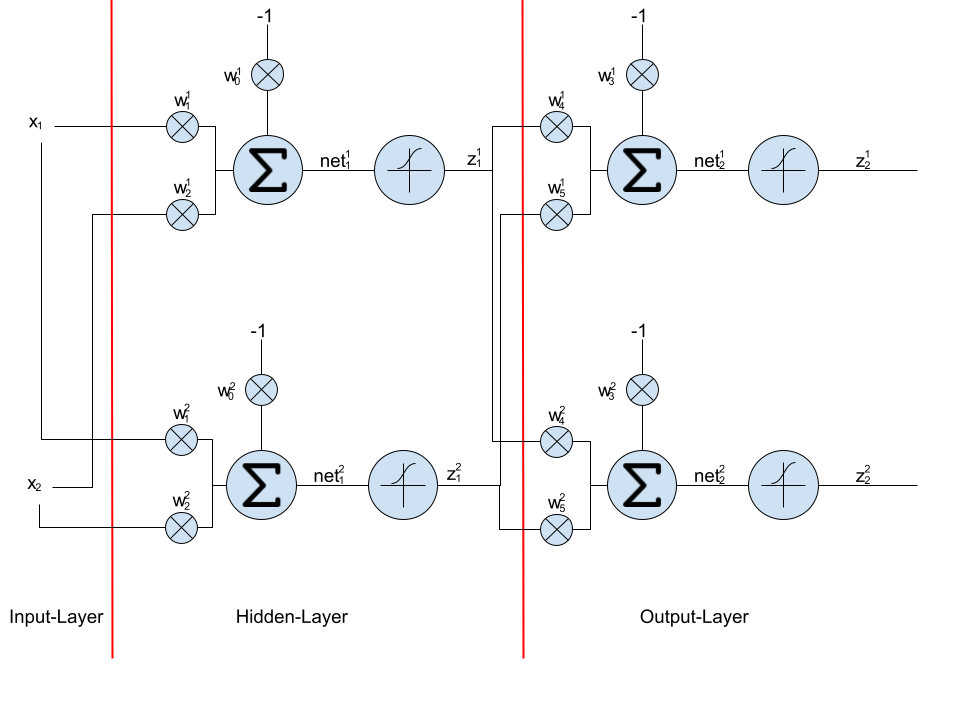
\includegraphics[width=1\linewidth]{../common/01_neuronal_network/00_resources/02_neuronales_netz.png}
    \end{center}
    \caption{Ein neuronales Netz mit einem Hidden-Layer}
    \label{fig:07_neuronal_network}
\end{figure}

\subsection{Lernverfahren mit Gradientenabstieg}

\subsection{Lernverfahren mit Backpropagation}

\subsection{XOR und die Lösung}